%!TEX root = ../thesis_a4.tex

\chapter{Music corpus and datasets}\label{chap:datasets}

\section{Introduction}
\label{sec:corpus_intro}

Data is a fundamental requirement in the development of information retrieval technologies~\citep{manning2008introduction}. A research corpora is a collection of data compiled to study a specific research problem. A well designed research corpora is representative of the domain under study used for the development and evaluation of approaches. It is practically infeasible to work with the entire universe of data. Therefore, to ensure the scalability of information retrieval technologies to real-world scenarios, it is to important to develop and evaluate the approaches using representative data corpus. In addition to catering the scalability of the approaches, an easily (or, better publicly) accessible data corpora provides a common ground for researchers to evaluate their methods, and thus, accelerate the advancement of the knowledge. 

Not every computational task would require an entire reseach corpus for development and evaluation of approaches. Typically a subset of the corpus is used in a specific research task. We call this subset a test corpus or test dataset. Test dataset is a static collection of data specific to an experiment, as opposed to a research corpus, which is an evolving collection of data. Therefore, different versions of the test dataset used in a specific experiment should be retained for ensuring the reproducibility of the results. The models build over test dataset can later be extended to entire research corpus. Note that a test dataset should not be confused with the training and testing split of a dataset often performing in a cross validation experimental setup.

In \gls{mir} a considerable number of the computational approaches follow a data-driven methodology, and hence, a well curated research corpora becomes a key factor in determining the success of these approaches. Due to the importance of a good corpora in research, building a corpora in itself becomes a fundamental research task. It has been studied in many fields such as XXX, XXX and XXX. \Gls{mir} is relatively a new research area within information retrieval, which has primarily gained popularity in last 2 decades. Even today a majority of the studies in \gls{mir} use an ad-hoc procedures to build a collection of data to be used for the experiments. Quite often the audio data comes from the researcher's personal music collection. Availability of a good representative research corpora has been a challenge in \gls{mir}. This to an extend can be attributed to the large variety of research problems studied within \gls{mir}, lack of standardized methodologies for data collection and annotation, and most of all, the constrained posed by the copyrighted content.

Recently there have been some efforts to compile large collections of music related data to build a research corpora that can be used to study a number of computational tasks in \gls{mir}. One such example is the Million Song Dataset (MSD)\TODO{ref}, which has been used in a number of studies for a variety of tasks\TODO{ref}. However, owing to the copyright issues, the audio for the recordings in MSD is not available. Building a good representative research corpora, which in the field of \gls{mir} would typically mean compilation of a large number of music recordings and it's related metadata is a big effort. A successful sustainable strategy could be to make it a community effort. An endeavor in this direction is AcousticBrainz\TODO{ref}, which aims to crowd source acoustic information for all music in the world and make it available to the public. Data in Acousticbrainz is indexed by unique MusicBrainz identifiers. MusicBrainz\TODO{ref} is an open music encyclopedia that collects music metadata and makes it available to the public. Such open repositories can also serve as corpora for a variety of research problems in \gls{mir}. 

\TODO{Mention COFLA somewhere}

While there is a growing effort towards building and using a representative sizable corpora in research, there are not many studies that address formally the task of building a good research corpora. There is a lack of studies that discuss the criterion for determining the goodness of a corpora for a particular task and systematic ways to compile and curate research corpora. Some recent efforts towards this direction includes the work by XXX in which the author present unified ways to describe annotated \Gls{mir} datasets. There have been some efforts to define a specifications to store annotations in a more unified way to promote reproducibility and easy access of the corpora. As a part of CompMusic project in XXX presents a set of design criterion for building research corpora that is representative of a given domain of study. These criterions are based around considerations such as purpose, coverage, completeness, quality and reusability. 

%The corpus developed in the CompMusic project for studying a number of problems in \Gls{mir} of \Gls{iam} is based on these criterion.

In this chapter we describe the CompMusic research corpora built for studying a number of computational tasks in \gls{mir} of \gls{iam}. Along with the description of the corpora we also briefly discuss the methodology  and the design criterion used to compile and curate the corpora. Note that the sources used for compiling the corpora are not comprehensive. Our primary aim is to present the approach we used to build the corpus than to justify a specific data source. In addition to the CompMusic corpora we also briefly describe the individual test datasets (Section XX) built for studying specific aspect of melody in \gls{iam}. These test datasets are used for evaluating different approaches described in subsequent chapters. 

The compilation of the CompMusic Corpora is a collective effort by the CompMusic team\TODO{ref}. This task mainly involved defining the criterion for selecting music material, procurement of the audio recordings, entering the associated editorial metadata in to MusicBrainz, organizing and maintaining collections on the disk, and correcting erroneous metadata fields by taking help from experts. Contributions have been made in all these tasks and mainly in the creation of the Hindustani music Corpus. The description of the CompMusic Corpora given below is based primarily on the work presented by~\cite{CM_Corpora_Ajay14,serra:14:corpus}.

%
%\begin{itemize}
%	\item Data is needed for dev of MIR approaches
%	\item MIR is primarily a data driven field
%	\item How should be the research corpus used for these approaches
%	\item What are the components of these corpus, how its used, in which modes
%	\item How does it develop
%	\item How is it curated/selected/ what should be the criterions. 
%	\item Issue of reproducibility in research, sharable corpus, open access corpus
%	\item examples of researhc corporas 
%	\item openly available corporas
%	\item ways to access them
%\end{itemize}


\section{CompMusic corpora}

As described earlier in Section XXX, in CompMusic project we work on data-driven computational approaches to describe music recordings and emphasize the use of domain knowledge of a particular music tradition. This project focuses on five different music traditions: Arab-Andalusian (Maghreb), Beijing Opera (China), Turkish makam music (Turkey), Hindustani (North-India) and Carnatic (South-India) music. One of the key ideas in CompMusic project is that there are some universal music concepts such as melody and rhythm common across different music traditions, but many important aspects of a music recording can be better understood and appreciated by focusing on the specificities of the music tradition. Therefore, a significant effort in this project has been to compile a representative research corpora that captures the specificities of different music traditions considered in the project. In addition, an effort is made to define the design criterion that can be used to build good research corporas. In the subsequent section we enumerate the criterion chosen to build the CompMusic corpora.

\subsection{Criterion for Creating Corpora}
\label{sec:corpus_criterion_for_corpora}

\cite{serra:14:corpus} enumerates a set of criterion for building a good representative research corpora that have been used in the CompMusic project. These criterion are listed below along with a brief description.

\subsubsection{Purpose}

The purpose for building a corpora should be clearly specified, which includes defining the research problem that needs to be addressed and the research approach that will be used. In CompMusic we want to develop methodologies to extract musically meaningful features from audio music recordings, primarily related to melody and rhythm. The approaches taken are based on signal processing and machine learning techniques. A research corpus should take these factors into account.

\subsubsection{Coverage}

As mentioned above, a good corpus should be representative of the domain under study. Coverage is a measure for the representativeness of a corpus with respect to the concepts to be studied. Given the quantitative approach of the CompMusic project, we need sufficient instances of each concept for the data to be statistically significant. For melodic analsis, we need to have audio recordings and appropriate accompanying information that represent the diversities present in the melodic aspects of Hindustani and Carnatic music such as different forms, artists from different schools of music, and the variety of \glspl{raga} frequently performed in each music culture. 

\subsubsection{Completeness}

To successfully use data in a meaningful analyses it should be complemented by the appropriate metadata. Completeness indicates the completeness of the metadata for each audio recording. For the CompMusic corpus it mainly refers to the completeness of the editorial metadata and of the descriptive information accompany each audio recording. 

\subsubsection{Quality}

The quality of the data in a corpus should be good. In our case it means that the audio has to be well recorded and the accompanying metadata should be accurate. We use commercial produced well recorded audio data and the accompanying information is obtained from reliable sources. Quite often the information collected from reliable sources such as editorial metadata on the CD cover is erroneous, in such cases the metadat is validated by experts. 

\TODO{Write a paragraph on the quality and the storing format of the audio collection}

\subsubsection{Reusability}

Reusability of the corpus is fundamental for reproducibility of the research results. An important aspect that impacts reusability is the ease of access to the corpus. This implies that the corpus should be available for the community to access and it has to be well structured for an easy integration. We address reusability by emphasizing the use of open repositories that are either already suitable or can be easily adapted to our needs. For organizing editorial metadata we use MusicBrainz. In addition, we make efforts for an each access of the corpus through the Dunya API.

\TODO{Explain the resuability component of the corpora, explain dunya API and ways to access data etc. Also emphasize the sharing and public availability of the datasets}




%\begin{itemize}
%\item the kind of research done in compmusic
%\item important of a good corpora in this project
%\item design principles followed for building this corpora
%\item Issue of open access, that makes it more powerful
%\item Structured way to access the corpora, through APIs
%\item Complemented by metadata for overall approaches and incorporating domain knowledge
%\item describing specific Hindustani and carnatic Datasets along with thir attributes and measurement of different parameters used to measure a good corpora.
%\end{itemize}


We now proceed to describe the specificities of the Carnatic and the Hindustani music corpus, both of which are a part of the CompMusic corpus. We will describe the data that constitute the corpus, the unit of the data sample, references for measuring completeness and coverage of the data, resources for obtaining complementary information about musical concepts and XXX. 


\subsection{Carnatic music corpus}
\label{sec:corpus_carnatic_music_corpus}

\Gls{raga} is the melodic and \gls{tala} is the rhythmic frameworks in both Carnatic and Hindustani music~(Section~XXX). They are the two key musical concepts in \gls{iam} around which the entire music is composed, performed, organized and taught. As a result of which these concepts have been the main considerations based on which both the corpora are compiled. Both the corpora primarily comprise audio recordings and its associated editorial metadata and are the ones used by signal processing and machine learning approaches. In addition to that there are lyrics, scores, contextual information on music concepts and community (social) information from online music forums and other sources.

There are several music tradition specific considerations taken into account while building the corpus. A concert, also referred as a (Kach\={e}ri), is the natural unit of Carnatic music. It is the unit typically considered in organization and digital distribution of Carnatic music content. Though Carnatic music is improvisatory in nature, it is predominantly based on compositions. Most of the compositions are to be sung, as a result of which, vocal music is dominant in Carnatic music. Even in instrumental music, the lead artist aims to mimic the vocal singing~\citep{Viswanathan2004}. Based on these considerations, we consulted expert musicians and musicologists, such as T.~M.~Krishna to arrive at a representative audio collection of Carnatic music.

The main institutional reference for gathering the Carnatic music collection is the \gls{mma}. The \Gls{mma} was conceived to be the institution that would set the standard for Carnatic music. Since 1929, the \Gls{mma} hosts annual conferences on music, which has eventually lead to the December music festival of Madras, one of the largest cultural events of the world. The \gls{mma} has been driving the scholarly research in Carnatic music since a long time and has influenced the evolution of the musical concepts being used. The \gls{mma} has an expert pannel that sets the standards and fix procedures for selecting artists for the music festival. Since a long time the \gls{mma} has been recording Carnatic music performances and its archive is considered as one of the main references for Carnatic music. However, the archive is not openly available online. We therefore procured the audio recordings through other commercial sources while following the musical criterion used by the \gls{mma}. We started by collecting the releases of the artists who have performed in the \gls{mma} in the last five years. Subsequently, we expanded the collection to include their teachers and other musicians popular in their era. 

One of the main record labels that specializes in Carnatic music recordings is Charsur, which has been publishing high quality commercial CDs for over 15 years now. The core of the Carnatic music audio collection is from their catalog of music concerts. The details of the Carnatic music corpus in terms of the unique number of recordings, releases, artists, \glspl{raga}, \glspl{tala} and compositions is shown in Figure~\ref{fig:carnatic_corpus_details}. In total, we have XXX number of vocal concerts and XXX number of instrumental concerts spanning XX hours of audio data.

\begin{figure}
	\begin{center}
		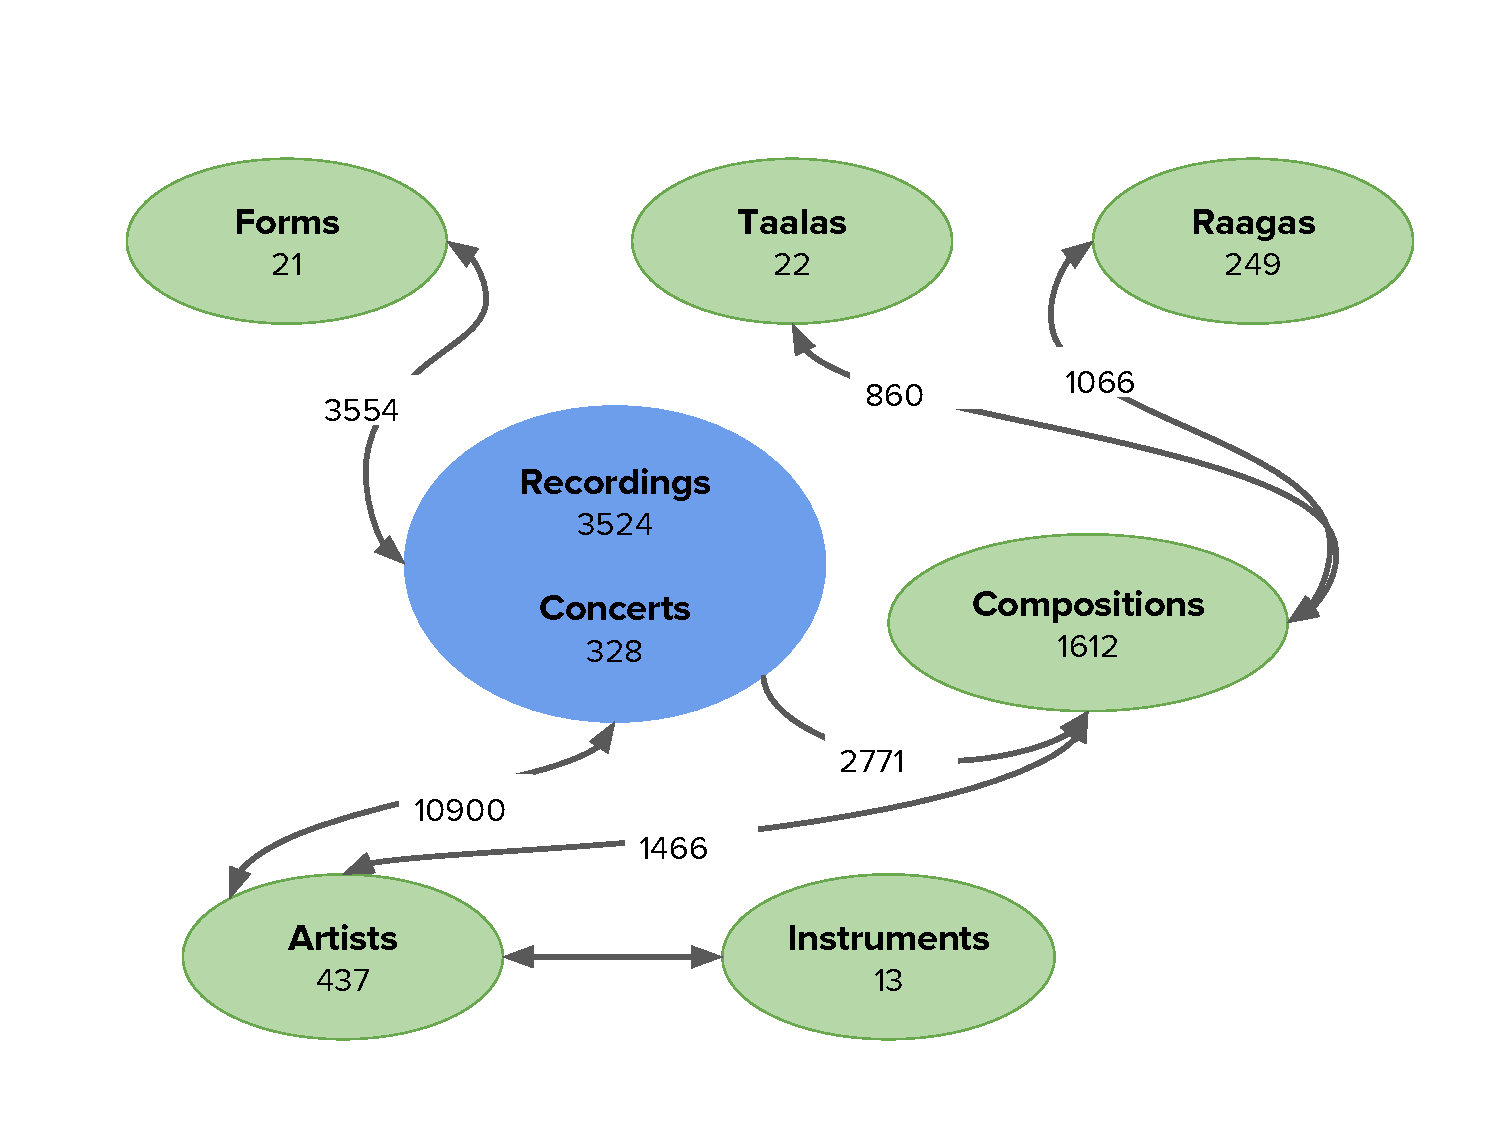
\includegraphics[width=\figSizeHundred]{ch04_datasets/figures/carnatic_corpus.pdf}
	\end{center}
	\caption{Details of the Carnatic music corpus in terms of the number of different musical entities and relationships between them.}
	\label{fig:carnatic_corpus_details}
\end{figure}

As mentioned before, since vocal music constitute a significant part of Carnatic music and that the music is largely based around compositions, lyrics play an important role. Scores on the other hand have a limited usability as the music is primarily improvisatory in nature. Nonetheless, for some computational analyses lyrics and scores might be useful, and hence, we make an effort to compile a small collection of them. For most of the currently performed compositions there exists several published compilations of lyrics and scores~\TODO{ref}, for example the ones by the three most recognised
composers; Tyagaraja [20], Syama Sastri [21] and Dikshitar
[22]. However, this data is not available in machine readable format and hence can't be used directly in computational analysis. There are some good open repositories of lyrics such as sahityam.net\TODO{ref} that provides lyrics in machine readable format. Sahityam.net is considered as a wikipedia of lyrics of Carnatic music and is our primary source for lyrics. It currently hosts lyrics for about 1820 compositions of Carnatic music. To the best of our knowledge there are only a few sources of music scores for Carnatic music that provide scores in machine readable format. A compilation of cores done by Dr. Shivkumar Kalyanaraman is our main source of scores for Carnatic music.

In addition to the signal processing and machine learning based approaches for which we primarily collected audio recordings and accompanying metadata, semantic analysis of \gls{iam} has been another topic of research. The music community and music concept related information collected from various sources over the Internet comprise the input data to semantic anlaysis and is a part of the Carnatic music corpus\TODO{ref}. Kutcheries.com and Wikipedia are two sources utilized for obtaining such an information. Kutcheries.com is a good source of artist biographies and information about music venues, concerts and other related events. The category of Carnatic music on Wikipedia is a good source of contextual information including music concepts. There has also been an effort to contribute to Wikipedia by adding information with the help of experts. In addition to these two sources more opinion like data on different musical aspects is obtained from Rasikas.org, an active music forum dedicated to Carnatic music community. In the case of Carnatic music the data from rasikas.org can be considered as ideal for studying tasks such as community profiling \TODO{ref}.


\subsubsection{Coverage of Carnatic music Corpus}
\label{sec:corpus_coverage_of_carnatic_music_corpus}

As mentioned before in Section~\ref{sec:corpus_criterion_for_corpora}, coverage analysis of a corpus aims to measure the representativeness and comprehensiveness of a corpus with respect to the reference sources that represent the real-world collections. For the case of the Carnatic music corpus coverage analysis is performed for \glspl{raga}, \glspl{tala}, performing artists and composers. The main reference sources we have considered for coverage analysis is Kutcheris.com, Charsur and Raaga.com. Kutcheris.com is our primary source for measuring artist coverage since it is up-to-date with current artists and their performances. We use last 5 years of their concert listing from 2009-2014. Release catalog from Charsur, our main reference as a record label also provides information about \glspl{raga}, \glspl{tala}, artists and composers. Raaga.com, an Indian music streaming service with a channel dedicated to Carnatic music is another source we considered for this analysis. It should be noted that Raaga.com has several light music forms included in their Carnatic music channel, which we have purposefully not included in our corpus. Hence, the numbers derived from an analysis done on the data from Raaga.com will have an adverse influence because of these additional music forms. The procedure followed for obtaining information from these sources and the post-processing done before the analysis is explained in the article by~\cite{CM_Corpora_Ajay14}.

For each music entity we define a coverage measure, the \textit{overlap} ($O$) as:

\begin{equation}
	O_{e}^{r} = \frac{ | S_{e}^{c} \cap S_{e}^{r} | }{ | S_{e}^{r} |}
	\label{eq:coverage_measure}
\end{equation}

\noindent where $O_{e}^{r}$ is the \textit{overlap} measure of the musical entity $e$ with respect to the reference source $r$, $S_{e}^{c}$ is the set of entities in the corpus and $S_{e}^{r}$ is the set of entities in the reference source. $|S|$ denotes the cardinality of a set $S$. In Table~\ref{tab:coverage_summary_carnatic_corpus} we summarize the coverage of the musical entities along with the overlap measure with respect to the reference sources mentioned above. We see that the coverage of the \glspl{raga} in the corpus is satisfactory and of the \gls{tala} is good. For composers and artists the numbers are low for Raaga.com, which can be attributed to the presence of light Carnatic music forms in their database. 

\begin{table}
\begin{centering}
\begin{tabular}{ c c c c c }
	\hline
					 & Corpus	& Raaga.com			& Kutcheris 	& Charsur\\
	\hline
	\Glspl{raga}	& 	246		& 	489 (42\%)		& 	N/A			& 301 (68\%)\\
	\Glspl{tala}	& 	18		& 	16 (100\%)		& 	N/A			& 21 (85\%)\\
	Composers		& 	131		& 	598 (17\%)		& 	N/A			& 256 (42\%)\\
	Artists			& 	233		& 	501				& 	2978		& 264 (48\%)\\						
	\hline
	
\end{tabular}
\par \end{centering}	
\caption[Coverage of the Carnatic music corpus]{Summary of the coverage of the Carnatic music corpus. The numbers in the paranthesis indicate the computed \textit{overlap} measure. N/A denotes data not available.} 
\label{tab:coverage_summary_carnatic_corpus}
\end{table}

Not all the performing artists in the corpus (Table~\ref{tab:coverage_summary_carnatic_corpus}) are lead artists. Among these 233 artists 74 are lead artists (lead vocal or lead instrumental), 28 are accompanying violinists and 48 are percussionists. Since Carnatic music corpus predominantly comprise vocal music, coverage of lead or vocal artists becomes more important. Also not every lead artist is equally popular, that should also be a consideration in measuring the representativeness of the corpus. The concerts listed by Kutcheris.com span the whole year and all through the day. However, the evening concerts are more
recognized, and we took it to be a measure of popularity of the artists. For a better coverage analysis, we thus consider three categories of artists: Artists-Set-1 (all the artists), Artists-Set-2 (artists who have performed in the evening concerts, through the year) and Artists-Set-3 (artists who
have performed in evening concerts between November and January). Of the 2978 total artists present in Set-1 on Kutcheris.com concert listings, there are 1814 artists in Set-2 and 1472 artists in Set-3.

\begin{figure}
	\begin{center}
		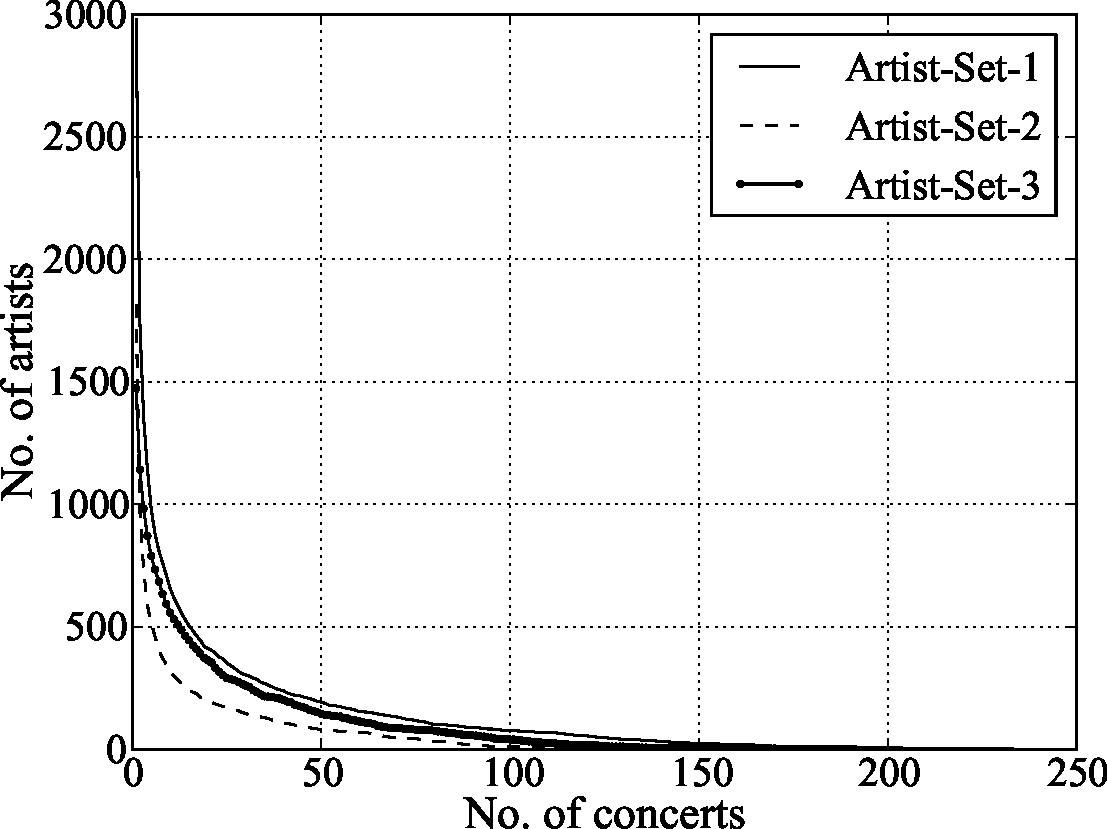
\includegraphics[width=\figSizeHundred]{ch04_datasets/figures/performances-vs-artists.pdf}
	\end{center}
	\caption{The number of artist by the number of their concerts. These artists are the ones obtained from Kutcheris.com}
	\label{fig:number_artrist_vs_number_concerts}
\end{figure}

In addition to the timing of the concerts, popularity of an artist can also be measured based on the number of concerts performed. Though there are a large number of artists listed in Kutcheris.com, we see that the distribution of the number of concerts they have performed is exponential (Figure~\ref{fig:number_artrist_vs_number_concerts}). We see that there are only about 200 artists of 2978 artists who have performed in over 50 concerts. To consider this aspect while measuring coverage, we compute the \textit{overlap} as defined in Equation~\ref{eq:coverage_measure} through different subsets of the artists in Kutcheris.com, sweeping over the number of concerts they have performed. Furthermore, we perform this analysis for different categories of the artists in the corpus as mentioned above.

\begin{figure}
	\begin{center}
		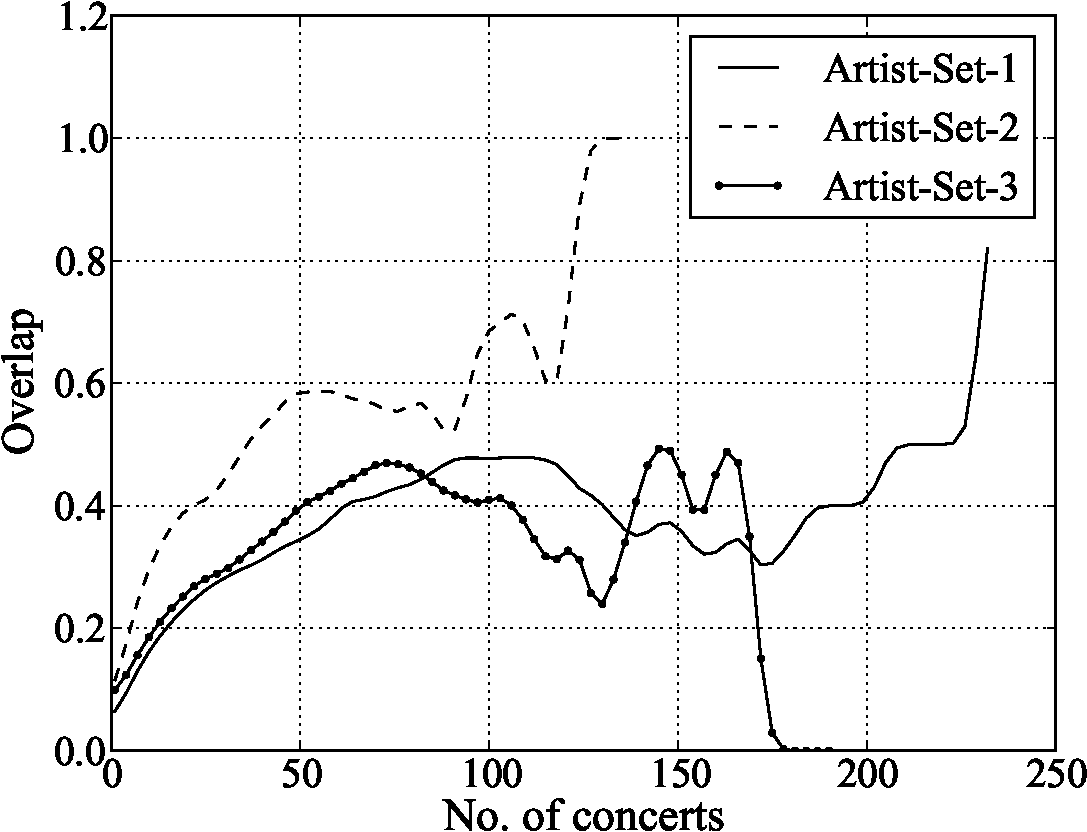
\includegraphics[width=\figSizeHundred]{ch04_datasets/figures/artist-coverage-vs-performances.pdf}
	\end{center}
	\caption{The \textit{overlap} between the artists in the corpus and those listed in Kutcheris.com for different artist sets determined by the number of performed concerts. The analysis is performed for category of artists in the corpus.}
	\label{fig:artist_coverage_vs_number_of_concerts}
\end{figure}

In Figure~\ref{fig:artist_coverage_vs_number_of_concerts} we show the \textit{overlap} between the artists in the corpus and the ones listed in Kutcheris.com for different sets of artists based on the number of performed concerts. We show the \textit{overlap} curve for all three categories of the artists in the corpus. We notice that the \textit{overlap} increases as we consider more frequently performing artists. We also observe that the \textit{overlap} saturates and becomes constant. This can be attributed to the fact that the most frequently performing artists are the accompanists and they are few in numbers compared to the lead artist, since they accompany multiple lead artists. Since the number of artists with more than 150 concerts is less, the \textit{overlap}
values becomes unreliable. Overall we notice that the \textit{overlap} is better for artists in the categories Artist-Set-2 than Artist-Set-1 and Artists-Set-3. This shows that the corpus has a better coverage of the artists from evening concerts round the year.

\subsubsection{Completeness of the Canatic Music Corpus}
\label{sec:corpus_completeness_of_completeness_of_carnatic_music_corpus}


As defined earlier, completeness of the corpus in the context of CompMusic corpora refers mainly to the completeness of the associated metadata
for each recording, which basically is obtained from MusicBrainz. There can be multiple reasons for the missing and the erroneous editorial metadata in the MusicBrainz. Many times commercially released CDs do not provide all the relevant editorial metadat on the cover-art. In several cases there is no mention of the accompanying artists or of the \gls{raga} and \gls{tala} of the musical piece in the CD. Very often composition information is missing on the CD cover. Another reason for incomplete metadata can be that the editorial metadata is not completely entered into MusicBrainz. This happens quite frequently for the fields such as recording relationships. Several times the metadata entered is erroneous. This is either due to a mistake done by the person uploading the metadata into MusicBrainz or the editorial metadata provided on the CD cover itself is wrong. Multiplicity of languages used in Carnatic music further adds to these inconsistencies. There has been some effort to automatically complete the missing metadata based on the relationships on the release or the recording using semantic web approaches\TODO{ref}. The missing metadata due to transliteration errors also has been addressed to an extent by making curated list of entities such as \gls{raga} and \gls{tala}, and using robust algorithm for matching and linking metadata\TODO{ref}. Despite these efforts, there are a significant number of recordings and releases for which the metadata is incomplete.


\begin{table}
	\begin{centering}
		\begin{tabular}{ c c c c}
			\hline
			Metadata	 		&  \#Recordings	& completeness (\%)\\
			\hline
			Lead artist			& 	1650	& 	100	\\						
			Accompanying artist	& 	1221	& 	74	\\
			\Glspl{raga}		& 	959		& 	58	\\
			\Glspl{tala}		& 	917		& 	56	\\
			Work (compositions)		& 	989		& 	60	\\
			
			\hline
			
		\end{tabular}
		\par \end{centering}	
	\caption[Completeness of the Carnatic music corpus]{Completeness of the Carnatic music corpus showing the number of recordings for which the corresponding metadata is available and the percentage (\%) of such recordings. The percentage values are rounded off to the nearest integer.} 
	\label{tab:completeness_carnatic_corpus}
\end{table}


In Table~\ref{tab:completeness_carnatic_corpus} we show the completeness of the recordings in the Carnatic music corpus. We see that all the recordings are at least labeled with a lead artist, but about a quarter of the recordings (429/1650) do not have accompanying artist information. \Gls{raga}, \gls{tala} and work (composition) labels are available for more than half the number of recordings. Note that there are several recordings that have the required editorial metadata but deemed incomplete because the names could not be accurately matched to any entity in the curated list. 


  
%
%\begin{itemize}
%	\item contents of the corpus
%	\item Considerations in collecting data/music recordings
%	\item whom we consulted how we went ahead for 
%	\item Academic references
%	\item Recording label, purchasing of material
%	\item storage of data
%\end{itemize}


\subsection{Hindustani Music Corpus}
\label{sec:corpus_hindustani_music_corpus}

Similar to the case of Carnatic music, \gls{raga} and \gls{tala} are the fundamental music concepts with which to describe melodic and rhythmic aspects of Hindustani music. They thus become the primary considerations while building the Hindustani music corpus as well. For Hindustani music also vocal music is predominant. However, compared to the Carnatic music the instrumental music is much more popular and prevalent. Hindustani music tradition as compared to Carnatic music is much more diverse and heterogeneous. One of the reasons for this can be the geographical spread of this music tradition. It thus presents a significant challenge in compilation of a good research corpus. Another major different between the two music traditions is that in Hindustani music the compositions are very short. These compositions basically act as base for improvisation, which is the main focus in a performance of Hindustani music. For the Hindustani music corpus we focus on two important vocal music styles; Dhrupad and Khy\={a}l. A Khy\={a}l performance typically has a lead vocals, a melodic accompaniment (typically given by harmonium or s\={a}ra\o{n}gi), a rhythm accompaniment (typically given by tabla) and a drone sound in the background (typically given by a t\={a}npura). 

There are many institutions that have compiled large audio archives of Hindustani music. The prominent ones among them are the ITC Sangeet Research Academy (ITC-SRA), Sangeet Natak Academy, and the All India Radio (AIR). Each of these institutions own thousands of hours of expert curated music recordings that represent the real world performance practice of Hindustani music. ITC-SRA is a premier music academy of Hindustani music and has taken up major efforts in the archival of music. Sangeet Natak Academy is India’s national academy for music, drama and dance. AIR is the largest public broadcaster in India and has a large archive of Hindustani music curated over many decades. AIR awards grades to musicians and its archives can be considered as a reference. None of these archives are publicly available. We gathered commercially released audio recordings from several music labels and compiled our corpus using these institutions as a reference. During this process we also consulted expert musicians and musicologists, such as Dr. Suvarnalata Rao at the National Centre for the Performing Arts (NCPA), Mumbai, India to curate the audio collection in the corpus. 

The Hindustani music corpus primarily comprises khy\={a}l and dhrupad vocal music releases, though a significant number of instrumental music releases are also present. There are 233 releases with a total of 1096 recordings spanning over 300 hours of audio. The details of the Hindustani music corpus in terms of the unique number of recordings, releases, artists, \glspl{raga}, \glspl{tala} and compositions is shown in Figure~\ref{fig:hindustani_corpus_details}.


\begin{figure}
	\begin{center}
		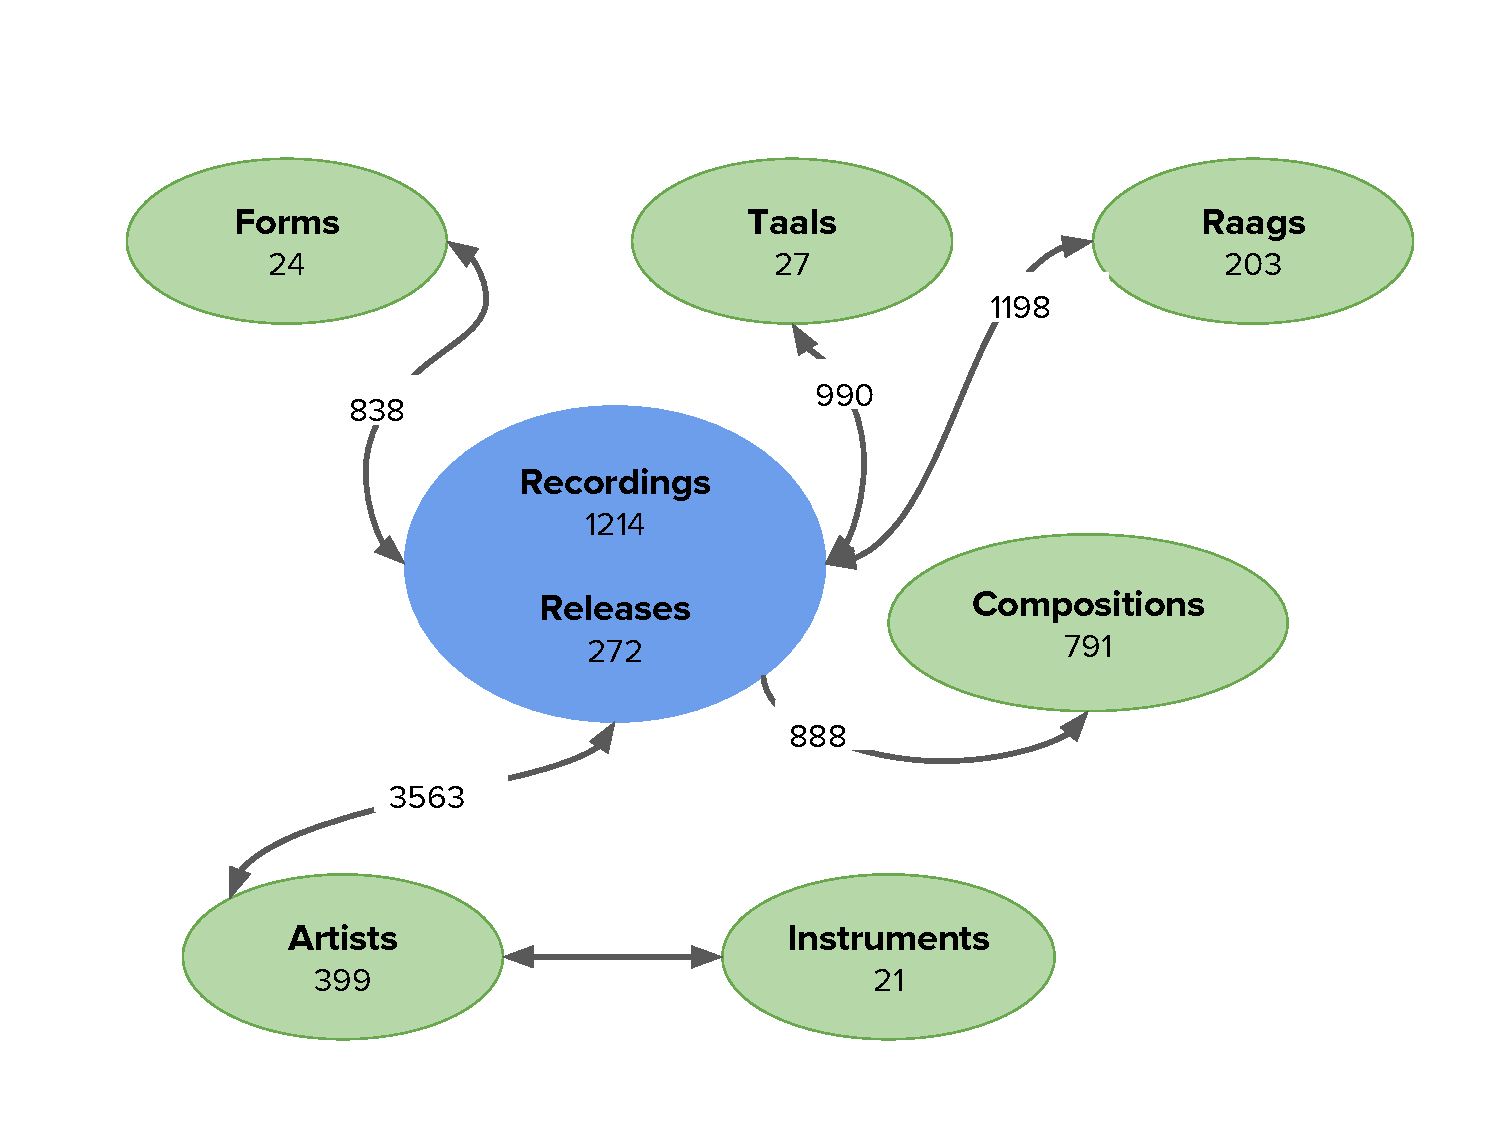
\includegraphics[width=\figSizeHundred]{ch04_datasets/figures/hindustani_corpus.pdf}
	\end{center}
	\caption{Details of the Hindustani music corpus in terms of the number of different musical entities and relationships between them.}
	\label{fig:hindustani_corpus_details}
\end{figure}


As mentioned before, compositions in Hindustani music are short and essentially act as base for improvisation. The music performances are mainly about improvisation. Due to these factors lyrics and scores are not very relevant for the computational anlaysis of Hindustani music. There exists a few repositories such as Bhatkhande\TODO{ref} and Ramashray Jha\TODO{ref} who have compiled lyrics and scores of several bandishes (compositions) using a standard notation for Hindustani music\TODO{ref}. However, they are not available in a machine readable format. In addition to lyrics and scores there are some information srepositories such as Swarganga Music Foundation \TODO{ref} for musical concepts such as \glspl{raga}, \glspl{tala} and bandishes. The category of Hindustani music on Wikipedia\TODO{ref} is a good source of contextual information including music concepts of Hindustani music.

\subsubsection{Coverage of Hindustani Music Corpus}
\label{sec:corpus_coverage_of_hindustani_music_corpus}

For the coverage analysis of the Hindustani music corpus we follow exactly the same methodology as was done for the Carnatic music corpus. The analysis is done for artists, \glspl{raga}, \glspl{tala} and compositions. Large geographical spread, lack of dedicated record labels and heterogeneous nature of the music make the coverage analysis of Hindustani music more complex compared to the Carnatic music. Therefore, it is challenging to do a comprehensive artist coverage analysis like the one presented for Carnatic music. For each of the entities we choose two main institutional references, ITC-SRA and Swarganga. In  Table~\ref{tab:coverage_summary_hindustani_corpus} we show the coverage of the Hindustani corpus. We see that even though the corpus and the chosen references are comparable in terms of the number of entities, the \textit{overlap} between them is less. This can be attributed to the differences in the purpose of creating the music collection. We mainly focused on recordings made in last 20-30 years to ensure good recording quality and to reflect current performance practices. On the other hand, both the references focus primarily on archiving Hindustani music and hence consist of several generations of artists, infrequent \glspl{raga} and \glspl{tala}, and a more comprehensive list of compositions. Furthermore, in our Hindustani music corpus we mainly focus on vocal music recordings of only two styles, khy\={a}l and dhrupad. The reference archives additionally include instrumental music and several other styles of Hindustani music.


\begin{table}
	\begin{centering}
		\begin{tabular}{ c c c c}
			\hline
			& Corpus	& ITC-SRA			& Swarganga\\
			\hline
			Artists			& 	360		& 	240 (19\%)	& 	629 (14\%)\\						
			\Glspl{raga}	& 	176		& 	185 (48\%)	& 	534 (13\%)\\
			\Glspl{tala}	& 	32		& 	N/A			& 	59 (37\%)\\
			Works			& 	685		& 	N/A			& 	1957\\

			\hline
			
		\end{tabular}
		\par \end{centering}	
	\caption[Coverage of the Hindustani music corpus]{Summary of the coverage of the Hindustani music corpus. The numbers in the paranthesis indicate the computed \textit{overlap} measure. N/A denotes data not available.} 
	\label{tab:coverage_summary_hindustani_corpus}
\end{table}


\subsubsection{Completeness of Hindustani Music Corpus}
\label{sec:corpus_completeness_of_hindustani_music_corpus}

In Table~\ref{tab:completeness_hindustani_corpus} we show the completeness of the editorial metadata for Hindustani music. We see that the editorial metadata for all the recordings at least includes the lead artist, and for more than half of the collection, the accompanying artists. Roughly 90\% of the corpora is annotated with the \gls{raga} label and more than half with the \gls{tala} label. Work (bandish) labels are present for nearly half of the collection. \={A}l\={a}p performances in Hindustani music are completely improvisatory musical pieces and are not based on compositions. Also, they are unmetered in nature, and hence they are not assigned any \gls{tala} label. Ideally, such music pieces should be discounted while assessing the completeness of the work  and the \gls{tala} metadata. Due to the unavailability of \={a}l\={a}p labels on recording these performances are also included in the assessment and hence work and \gls{tala} completeness is an underestimate.



\begin{table}
\begin{centering}
	\begin{tabular}{ c c c c}
		\hline
		Metadata	 		&  \#Recordings	& completeness (\%)\\
		\hline
		Lead artist			& 	1096	& 	100	\\						
		Accompanying artist	& 	658		& 	60	\\
		\Glspl{raga}		& 	960		& 	88	\\
		\Glspl{tala}		& 	627		& 	57	\\
		Work (Bandish)		& 	576		& 	53	\\
		
		\hline
		
	\end{tabular}
	\par \end{centering}	
\caption[Completeness of the Hindustani music corpus]{Completeness of the Hindustani music corpus showing the number of recordings for which the corresponding metadata is available and the percentage (\%) of such recordings. The percentage values are rounded off to the nearest integer.} 
\label{tab:completeness_hindustani_corpus}
\end{table}


\subsection{Open-access Research Corpus}
\label{sec:corpus_open_access_research_corpus}

The audio recordings compiled in both Hindustani and Carnatic music corpus as described above are taken from commercially released music CDs. These recordings are easily accessible, but owing to the copyright issues they can not be distributed freely and made publicly available. Therefore, even though re-compiling the corpus is theoretically possible, practically that would require a lot of effort from a researcher trying to reproduce the research results \TODO{rephrase this line, also we do share audio excerpts}. To promote the idea of open-access and reproducibility of the research results, in CompMusic project there has been an effort to compile an open-access music collection. This open-access corpus comprises both Hindustani and Carnatic music. Like the other research corpora described in previous sections, this corpus contains audio recordings and associated editorial metadata. In addition, this corpus also contains several annotations of different music attributes such as melodic phrases, sama locations and sections. Due permissions are taken from the artists for redistribution of the audio recordings, as a result of which the corpus is made publicly available under creative commons license (CC BY-NC 4.0). The audio recordings in this corpus are hosted on Internet Archive and made accessible through the Dunya API (Section XX). 



\begin{figure}
	\begin{center}
		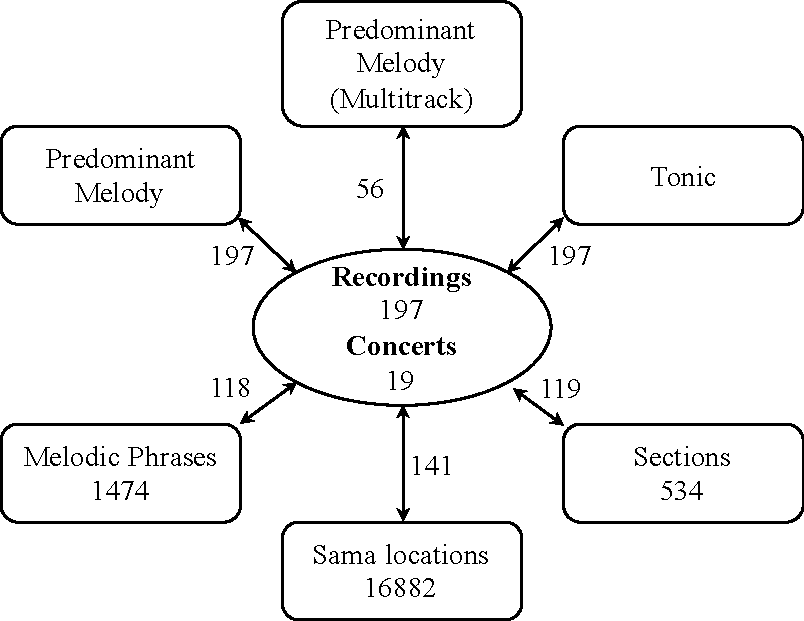
\includegraphics[width=\figSizeNinety]{ch04_datasets/figures/carnatic_CC_details.pdf}
	\end{center}
	\caption{Details of the Carnatic open-access music corpus in terms of the number of available annotations of different musical attributes and audio features.}
	\label{fig:carnatic_open_access_corpus_details}
\end{figure}


The Carnatic music part of the open-access corpus contains 19 releases, XXX number of recordings spanning XX hours of music. Majority of these releases correspond to Carnatic music concerts performed and recorded in Arkay Convention Center in Chennai, India. These are multi-track recordings later mixed and mastered by a professional. Individual music pieces of a concert are split into separate recordings, which then comprise a release. In addition to the content procured from Arkay, a number of releases in this corpus are commercially released CDs with artist's due permissions to make them publicly available. Along with the audio recordings and accompanying editorial metadata this corpus contains carefully done annotations corresponding to melodic, rhythmic and sectional aspects of the music. Manually done annotations include characteristic melodic phrases and sections within each audio recording. Semi-automatically done annotations include time-aligned sama locations and tempo in a recording. Finally, automatically done annotations, which can also be regarded as mid-level audio features include predominant pitch contour and tonic used the recording by the lead artist. Since several recordings are also available in multi-track, along with the predominant pitch estimated from the mixed track we also compute pitch of the solo vocal track. These pitch contours can serve as a ground-truth data to evaluate pitch tracking algorithms for \gls{iam}. In Figure XXX we show the number of available annotations of different musical attributes and audio features for the Carnatic music part of the corpus.


\begin{figure}
	\begin{center}
		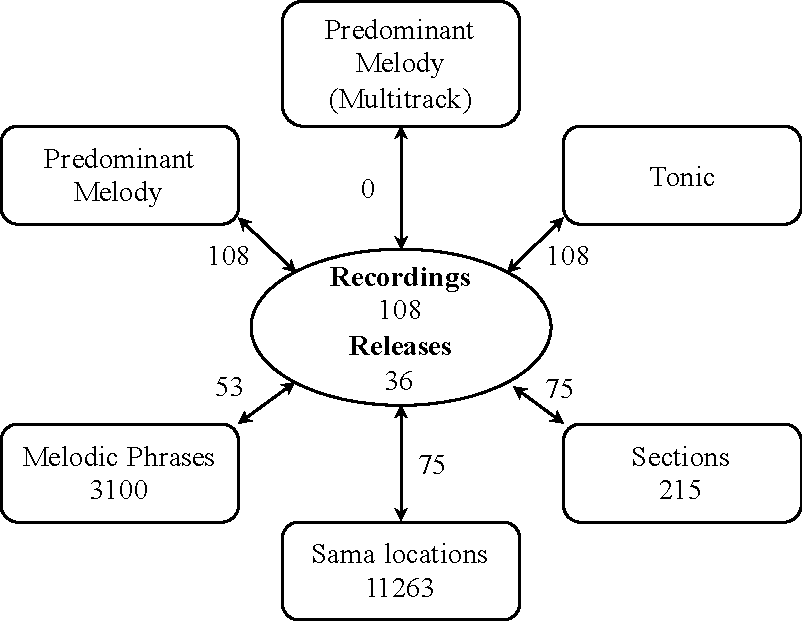
\includegraphics[width=\figSizeNinety]{ch04_datasets/figures/hindustani_CC_details.pdf}
	\end{center}
	\caption{Details of the Hindustani open-access music corpus in terms of the number of available annotations of different musical attributes and audio features.}
	\label{fig:hindustani_open_access_corpus_details}
\end{figure}

The Hindustani music part of the open-access corpus contains 32 releases, which has XXX number of recordings spanning XXX hours of music. A significant part of this collection comprises commercial releases by several maestros such as Pt. Ajoy Chakbraborty and Kumar Gandharva. The other part of the collection comprises individual recordings procured from different professional musicians and grouped together into releases per artist. The grouping is based on common performance practices clubbing the \glspl{raga} that are performed together in a concert. Hindustani open-access corpus also contains annotations for characteristic melodic phrases, sections, time-aligned sama locations and tempo. It also contain mid-level audio features including predominant pitch contour and tonic  frequency used in the recording. Since multi-track recordings are not procured for Hindustani music, like Carnatic music there are no pitch contours extracted from solo vocal track. In Figure XX we show the number of available annotations of different musical attributes and audio features of Hindustani music part of the corpus. 

\subsection{Storage and Access of Corpus}
\label{sec:corpus_storage_and_access}

The above sections described the Carnatic and the Hindustani research corpus compiled in the CompMusic project in terms of the design criterion and its coverage and completeness. In this section we provide details on the storage and the access of this corpus.

The audio corresponding to all the corpora describe above are stereo recordings sampled at 44.1\,kHz. Most of the audio recordings in the corpora are ripped from commercially release CDs. We compress and store the recordings as 160\,kbps MP3 files. The audio files for the open-access corpus are hosted on Internet Archive, and the rest are stored on the servers in Universitat Pompeu Fabra. In addition to audio the corpora contains different melody and rhythm related audio features such as predominant pitch contours, tonic of the recording and tempo. These features are stored along with the audio recordings on the university servers.

As mentioned before, for every single audio recording included in the corpus there is an accompanying editorial metadata. The metadata typically includes the following fields; lead artist, accompanying artist, instrument played by these artists, \gls{raga} and \gls{tala} of the music piece, music form and the name of the composition of the piece. For the case of Hindustani music it also includes the \gls{laya} information. All this metadata is structured and stored in MusicBrainz, an open music encyclopedia. Every concept in MusicBrainz has a unique identifier, which makes the processing of this metadata much easier. Typical issues arising from different spellings of an entity, different pronunciations and aliases is also avoided by using this schema. There are several other advantages of using MusicBrainz such as its ability to publish its database into Linked Data, mapping of entity concepts to Music Ontology, its REST-based webservice API for direct access to its data. Above all, its a community driven open-content initiative and has its majority of the data in public domain.

All the data associated with a recording; the audio file, extracted set of features and the accompanying metadata can be accessed through the Dunya platform. Dunya allows access to this data in two ways; through a web-based graphical interface and through a REST-based API interface. Dunya platform along with the details on how to access the data is provided in Section XXX. Note that though the data is accessible for research purposes after a user registration step, not all the data in the corpora is in public domain. \TODO{what more?}


%For researchers to be able to programmatically able to access the data, the second method is suited. Working with Dunya requires a user to first signup. Every user is then assigned a key, which can be used to authenticate the user while using the API. The documentation of the API can be found here. There is a



%Dunya system
%Dunya API
%Access features
%Who can access what ! Issue of being openly publicly available!


\section{Test Datasets}
\label{sec:corpus_test_datasets}

As explained earlier, a test dataset is a subset of a corpus used for studying a specific task. Typically these datasets are experiment specific and may contain additional information such as annotations. We here present the datasets that are used in this work for different computational melodic analysis tasks in \gls{iam}. Some of these datasets are quite generic and contain high quality comprehensive editorial metadata along with the audio recordings. And hence, we envision their usage in other melodic analysis tasks beyond the ones addressed in this dissertation.

Since a majority of these datasets are a subset of the corpora described in previous sections, details regarding the quality of the audio recordings and available editorial metadata remain the same as that of the corpora. In case of exceptions, these details are provided in the section where the dataset is described. 


\subsection{Tonic datasets}
\label{sec:corpus_tonic_datasets}


{\renewcommand{\arraystretch}{1.5}
\begin{sidewaystable} 
\begin{centering}
	\begin{tabular}{ c | c  c  c  c  c  c  c  c  c  c }
\tabletop
		Dataset 	&Avg. length (min)&\#Excerpts&	 	Hi.(\%) 	& 	Ca.(\%)	& 	Voc.
		(M/F)(\%) & Inst. (\%)	& 	\#Usong   	& 	\#Uartists	\\
\tablemid
		\acrshort{tds_cm1}		&3 &271	&	 41		& 	59	&	0			& 	100		& 	169		&	33	\\
		\acrshort{tds_cm2}		&3 &935	&	 45	 	& 	55	&	100 (68 / 32)		&	0		& 	547		&	81	\\
		\acrshort{tds_cm3}		&14.8&428	&	 45	 	& 	55	&	100 (72 / 28)		& 	0		&	428		&	71	\\
\hdashline
		\acrshort{tds_iitm1}		&144.6&38&	 0		& 	100	&	89 (79 / 21)		&	11		& 	N/A		&	22	\\
		\acrshort{tds_iitm2}		&12.3 &472	&	 0	 	& 	100	&	92 (77 / 23)		&	8		& 	472		&	22	\\
\hdashline
		\acrshort{tds_iisc}		&7.4&55	&	 0		& 	100	&	100 (80 / 20)		&	0		& 	55		&	5	\\
\tablebot
	\end{tabular}
	
	
	\caption{Summary of the tonic datasets, including average excerpt length (Avg. length),
		number of excerpts (\#Excerpts), percentage of Hindustani music (Hi), Carnatic
		music (Ca), vocal excerpts (Voc.), instrumental excerpts (Inst.), number of
		unique songs (\#Usong) and number of unique artists (\#Uartists) in each dataset. For vocal
		excerpts we also provide the breakdown into male (M) and female (F)
		singers. Percentage (\%) values are rounded to the nearest integer.}
	\label{tab:tonic_datasets}
\par \end{centering}	
\end{sidewaystable}

We use six different datasets with varied characteristics for the comparative evaluation of approaches for tonic identification task in in \gls{iam}. The comparative evaluation is presented in \chapref{chap:data_preprocessing} and is based on the work presented by~\cite{Gulati2014Tonic}. Some of these datasets also have an overlap with the datasets used for evaluation in our earlier studies~\citep{salamon2012multipitch,gulati2012two}. A summary of these tonic datasets in terms of different attributes of the comprising excerpts such as their average length, their total number, proportion of Hindustani/Carnatic, instrumental/vocal and male/female excerpts, and unique number of songs and artists is provided in Table~\ref{tab:tonic_datasets}. We now describe each of these datasets in detail. Note that three out of the six datasets; \acrshort{tds_cm1}, \acrshort{tds_cm2} and \acrshort{tds_cm3} are compiled as a part of the work in this dissertation. 


\subsubsection{CompMusic Tonic Datasets}
\label{sec:corpus_compmusic_tonic_dataset}

The first three datasets shown in \tabref{tab:tonic_datasets}; \acrshort{tds_cm1}, \acrshort{tds_cm2} and \acrshort{tds_cm3} are tonic datasets compiled as a part of the CompMusic project. They are derived from the Carnatic and the Hindustani research corpus described in the previous section. These datasets contain audio excerpts, associated metadata (lead artist, lead instrument, gender of the lead artist in case of a vocal performance) and tonic annotations. The main difference across these three datasets is in terms of the duration of the excerpts and the type of music performance (vocal vs instrumental). These datasets comprise a diverse set of artists and music material such as gender of the singer, set of \glspl{raga} and music forms. Due to the diversity of the datasets and the fact that these excerpts are taken from commercial releases, they can be regarded as a representative collection of \gls{iam} performances for tonic identification.  

\acrshort{tds_cm1} and \acrshort{tds_cm2} comprise three minute long audio excerpts extracted from full length musical performances of \gls{iam}. When the performance is longer than 12\,minutes, we extracted 3 excerpts from the beginning, middle and end of the recording. When the song was shorter than 12\,minutes only one excerpt from the beginning was extracted. By taking excerpts from different sections of a song we ensure that the datasets are representative, since the musical characteristics can change significantly between different parts of a recording. \acrshort{tds_cm1} contains exclusively instrumental performances, and does not overlap with \acrshort{tds_cm2} and \acrshort{tds_cm3}. The latter two contain exclusively vocal performances, where \acrshort{tds_cm3} contains full performances and \acrshort{tds_cm2} contains excerpts taken from the performances in \acrshort{tds_cm3}. 

The tonic pitch for the vocal performances and tonic pitch-class for the instrumental performances was manually annotated for each excerpt. All the annotations were later verified by a professional Carnatic musician and the number of discrepancies was very small and later corrected. To assist the annotation process, we used the candidate generation part of the approach proposed by \cite{Salamon2012}. For every excerpt the top 10 tonic candidates were synthesized together with the original audio file to help identify and label the correct candidate. Note that the correct tonic pitch was always present amongst the top 10 candidates. A detailed description of this procedure is provided in~\cite{SGulati_MThesis2012}.


\TODO{A figure of tonic values in 428 + 169 performances}
\TODO{How can we obtain this dataset}


\subsubsection{IITM Tonic Datasets}
\label{sec:corpus_iitm_tonic_datasets}

Datasets \acrshort{tds_iitm1} amd \acrshort{tds_iitm2} summarized in \tabref{tab:tonic_datasets} are compiled by~\cite{bellur2012knowledge}. These datasets were compiled by selecting 40 concerts from a private collection of hundreds of live concert recordings. These 40 concerts comprise 472 music
pieces of Carnatic music. In order to study the robustness of tonic identification methods,
the concerts that were selected range from artists from the 1960's to present
day artists. The quality of the recordings vary from poor to good, usually depending on the period in which they were made. \acrshort{tds_iitm1} comprises 38 of these concerts. \acrshort{tds_iitm2} comprises full length complete music pieces extracted from these 40 selected concert recordings. These performances are of varying duration, ranging from 46 seconds to 85 minutes. The tonic pitch for \acrshort{tds_iitm1} amd \acrshort{tds_iitm1} was manually annotated by a professional Carnatic musician.


\subsubsection{IISC Tonic Dataset}
\label{sec:corpus_iisc_tonic_dataset}

The \acrshort{tds_iisc} dataset is compiled by~\cite{ranjani2011carnatic}. It comprises audio recordings obtained from an online Carnatic music archive\footnote{\url{http://www.shivkumar.org/music/index.html}} compiled by Carnatic musician and enthusiast Dr.~Shivkumar Kalyanaraman, for the benefit of music amateurs and hobbyists as an online educational resource. The archive includes various forms of Carnatic music. \acrshort{tds_iisc} consists of 55 music pieces in the \gls{alapna} form, recorded by five singers across seven \glspl{raga}. The total duration of the dataset is 6.75\,hours. It includes recordings from the last 50 years, many of which were recorded live on analog audio tapes. The overall quality of the recordings is not very high. This makes it a challenging dataset for evaluating the accuracy of tonic identification task. The tonic pitch for this dataset was manually annotated by two professional musicians, S.~Raman and S.~Vijayalakshmi.


These six datasets represent the diversities present in real-world music collections of \gls{iam} in terms of the audio quality and music material, with which to study the task of automatic tonic identification. To the best of our knowledge these are the largest and most comprehensive datasets available for studying the task of tonic identification in \gls{iam}.

\subsection{Nyas dataset}

\subsection{Melodic similarity dataset}

\subsection{Raga recognition dataset}

\subsection{Saraga dataset}








